\chapter{Optimization and Control of a kHz Laser System} \label{ch:6}

The work of \autoref{ch:5} has illustrated the usefulness of machine learning methods in the field of ion acceleration and what sort of quantities might be optimized. To generate enough data for the \gls{ML} algorithms, the facilities need to use both a high-repetition rate laser (i.e. many shots per second) and a continuously refreshing target (e.g. a flowing liquid or tape drive target). Using such a system, no research group has yet obtained a stable and tunable MeV source of protons required for applications. Using a solid Kapton tape, Loughran et al. \cite{Loughran_2023_HPLSE} used \gls{BO} at \gls{RAL}, but only on around 60 bursts of shots. Using a flowing liquid target, multi-MeV deuteron acceleration \cite{Treffert_2022_APL} was demonstrated from a flowing liquid target at \gls{CSU}, but only operated over 2 minutes for a total of 60 shots.

At the Wright-Patterson Air Force Base, a 1 kHz, mJ class laser system exists that is capable of producing MeV protons \cite{Morrison_2018_NJoP}. In comparison to the two previously mentioned studies at \gls{CSU} and \gls{RAL}, a 1 kHz laser shoots one thousand to two thousand times more shots per second! A laser system that shoots one thousand times more shots per second, however, will also roughly have a thousand times less laser energy per shot. Morrison et al. \cite{Morrison_2018_NJoP} was able to achieve 2 MeV protons on this kHz system at \gls{WP-ELL}, while higher energy Hz laser systems can easily achieve tens of MeV. 

To enhance the MeV proton yield within the existing mJ class laser system, the \gls{TNSA} mechanism needs to be optimized as much as possible. This can be done in multiple ways:

\begin{itemize}
\item As explained in \autoref{ch:4}, multiple pulses can yield higher proton energies with the same amount of laser energy through \gls{eTNSA}. Even when the pulses are not spatially aligned, the preplasma induced from the first pulse can enhance the absorption in from the second pulse and yield higher proton energies as long as the rear side of the target is relatively undisturbed \cite{Macchi_2013_RevModPhys}. Relevant parameters here would be pre-pulse contrast, time delay between pulses, and a variety of other spectral properties of the pulse could even be optimized through the use of an instrument like the DAZZLER (see Loughran et al. \cite{Loughran_2023_HPLSE} for an example). 

\item Generally, thinner targets see enhanced proton acceleration via the vacuum heating mechanism which is a well known scaling captured in the Fuchs et al. \cite{Fuchs_2005_Nat} model explored in \autoref{ch:5}. However, targets that are too thin may break up before the acceleration takes place. Relevant parameters here would be the thickness, composition, and shape of the target. 
\end{itemize}
Evidently, many parameters influence the laser-target interaction in a very non-linear way which cannot be easily seen through the raw data. In this chapter, I give an overview of the kHz laser system at \gls{WP-ELL} and particularly focus on the \gls{DAQ} developed by fellow graduate student Nathaniel Tamminga and \gls{CSUCI} professor Scott Feister. Then, the code and machine learning framework that I developed, with some help from Jack Felice, to send optimized parameters back to the \gls{DAQ} is described. Finally, some results from this elementary machine learning feedback loop are discussed. The experimental operation of the laser was handled by the lab technician Kyle Frische. Miami University professor and former OSU graduate student Joseph Snyder helped with the experiments using his prior experience at the laboratory. Additionally, Anil Patnaik and Michael Dexter from AFIT and OSU professor Enam Chowdhury gave valuable feedback during weekly meetings for this effort. The results from this work are currently under consideration at \emph{APL Machine Learning}.

\section{Background}

In this section, I will describe the experimental setup at the \gls{WP-ELL} which uses a Ti:Sapphire based ultra-intense $780 \unit{\nano \meter}$ laser and a liquid sheet target.  

\subsection{Experimental Chamber}

With a maximum energy of $\sim 9 \unit{mJ}$, \gls{FWHM} period of $35 \unit{\femto \second}$, the \gls{WP-ELL} laser system is capable of producing pulses of peak intensity $\SI{5e18}{\watt \per \centi \meter \squared}$ with a 1.8 $\unit{\micro \meter}$ \gls{FWHM} spot size. By picking off a small amount of laser energy from the main pulse ($\sim \SI{12}{\micro \joule}$), an artificial pre-pulse can be used with a tunable delay between the pulses. Each of the beams are focused by an \gls{OAP}. These features are shown in \autoref{fig:experimental_chamber}. Additionally, a sequence of waveplates allows the main pulse and pre-pulse intensity to be reduced by up to a factor of ten by simply rotating the plate to a precise angle.

\begin{figure}
	\centering 
	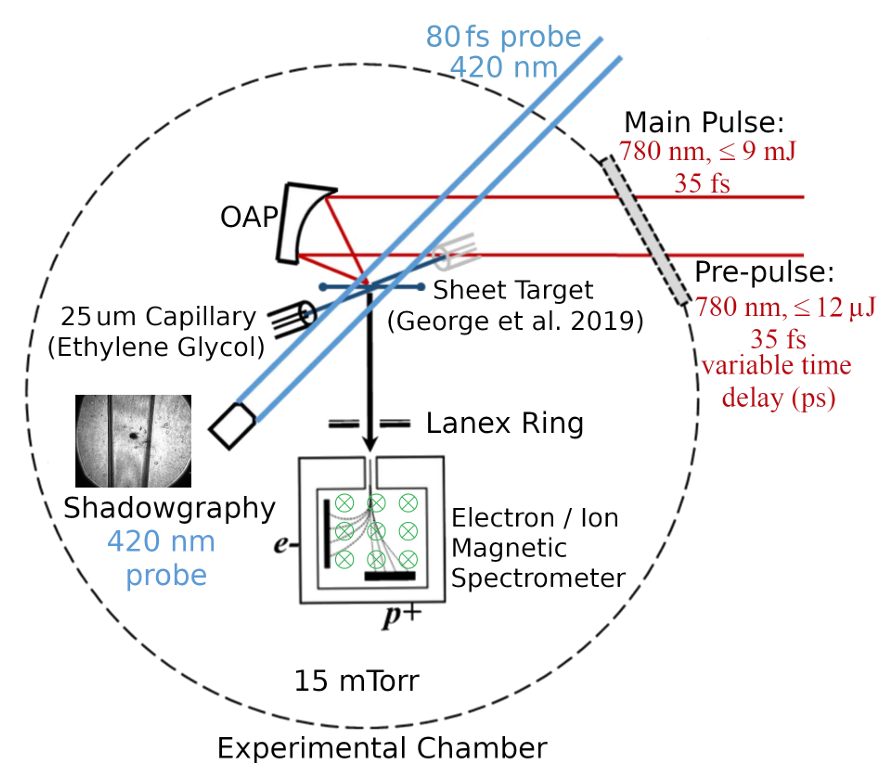
\includegraphics[width=0.75\linewidth]{planning/images/daq/experimental_chamber.PNG}
	\caption{A schematic of the experimental chamber, targetry system, diagnostics, and laser pulses entering the chamber at a kHz repetition rate. Figure taken from a manuscript in review by Tamminga et al.}
	\label{fig:experimental_chamber}
\end{figure}

The sheet target, described in detail in George et al. \cite{George_2019_HPLSE}, is formed by the grazing incidence of two extremely thin liquid stream of around 25 $\unit{\micro \meter}$ each. The target can be seen via shadowgraphy as seen in \autoref{fig:liquid_leaf}(A). The laser interaction with the sheet target can be seen in \autoref{fig:experimental_chamber} as the black dot in the center of the shadowgraph. We can see in \autoref{fig:liquid_leaf}(B) that the target has an oval shape which is why it is sometimes referred to as a ``liquid-leaf'' target \cite{Schmitz_2023_LaPB}. Since background particles are deleterious to the laser-matter interaction \cite{Snyder_2020_SciRep}, the chamber is pumped down to a pressure of 15 mTorr. Ethylene glycol is the chosen liquid in this experiment due to its ability to exist as a liquid at room temperature at these extremely low vacuum pressures, but other liquids (like $\text{H}_2\text{O}$ or $\text{D}_2\text{O}$) can be used as well at a possibly higher pressure.

\begin{figure}
	\centering 
	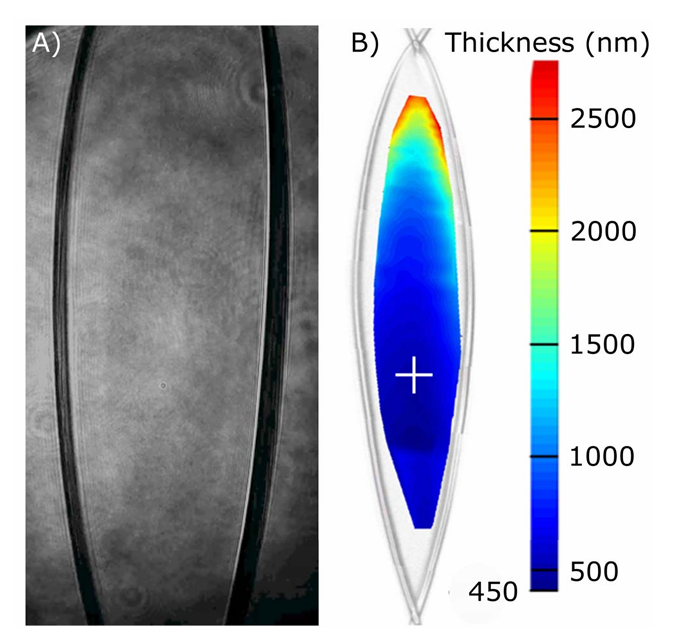
\includegraphics[width=0.75\linewidth]{planning/images/daq/target.PNG}
	\caption{(A) Microscope Shadowgraphy image of the central region of the liquid sheet target in vacuum. (B) Spatially dependent thickness map across the liquid sheet, collected with a Filmetrics white-light interference profiler. The white cross indicates the location of the minimum sheet thickness at 450 $\unit{\nano \meter}$. For scale, the width of the sheet in (B) is 560 $\unit{\micro \meter}$. A schematic of the experimental chamber, targetry system, diagnostics, and laser pulses entering the chamber at a kHz repetition rate. Figure reprinted from Figure 5 of George et al. \cite{George_2019_HPLSE}.}
	\label{fig:liquid_leaf}
\end{figure}

The electrons and ions accelerated normal to the rear of the sheet target travel through a Lanex Ring into the magnetic spectrometer: essentially a magnet that deflects negative particles to the left and positive particles to the right (in reference to \autoref{fig:experimental_chamber}). Using the fact that the cycltron radius of a charged particle in a magnetic field varies based on its velocity, the final location of the deflected particle determines its kinetic energy. The \gls{CCD} detectors are coated with scintillating material which converts the particle energy into a light signal that the \gls{CCD}s are capable of detecting.  

\subsection{Data Sources}

\subsubsection{CCDs}

The electron and proton spectra are collected from Mightex \gls{CCD} cameras. They each have 3648 pixels with $\SI{8}{\micro \meter}$ pixel width. As can be seen from \autoref{fig:experimental_chamber}, the higher energy particles should be reflected less and should (which translates to hitting the right end of the detector for electrons and the left end of the detector for positive ions). The magnetic field profile has been mapped out in previous work \cite{Morrison_2018_NJoP} so that a one-to-one correspondence between pixel location and kinetic energy can be established for both electrons and protons seen in \autoref{fig:pixel_energy}. 

The CCD pixels store counts up to 65,536 (unsigned 16 bit integer) which are collected over the desired exposure time. For example, if the Mightex cameras are set to collect at 100 Hz, they can have an exposure time of up to 10 ms. Pixels 0 to 900 for the proton CCD fall close to the direct line of sight of an undeflected particle and thus can receive stray signals from other radiation sources like x-rays. Since protons from this laser system have peaked at 2.5 MeV \cite{Morrison_2018_NJoP} (around pixel 1000), ignoring pixels 0 to 900 does not throw away any high energy proton data. Furthermore, 13 (additional) pixels are shielded from light which can be used to set a noise floor.

\subsubsection{Laser Diodes}

\section{Optimization Experiments}

\subsection{Automated Data Analysis}

\subsection{June 6, 2024}

\subsection{August 8, 2024}

\section{Conclusion}